% Options for packages loaded elsewhere
\PassOptionsToPackage{unicode}{hyperref}
\PassOptionsToPackage{hyphens}{url}
%
\documentclass[
]{article}
\usepackage{amsmath,amssymb}
\usepackage{iftex}
\ifPDFTeX
  \usepackage[T1]{fontenc}
  \usepackage[utf8]{inputenc}
  \usepackage{textcomp} % provide euro and other symbols
\else % if luatex or xetex
  \usepackage{unicode-math} % this also loads fontspec
  \defaultfontfeatures{Scale=MatchLowercase}
  \defaultfontfeatures[\rmfamily]{Ligatures=TeX,Scale=1}
\fi
\usepackage{lmodern}
\ifPDFTeX\else
  % xetex/luatex font selection
\fi
% Use upquote if available, for straight quotes in verbatim environments
\IfFileExists{upquote.sty}{\usepackage{upquote}}{}
\IfFileExists{microtype.sty}{% use microtype if available
  \usepackage[]{microtype}
  \UseMicrotypeSet[protrusion]{basicmath} % disable protrusion for tt fonts
}{}
\makeatletter
\@ifundefined{KOMAClassName}{% if non-KOMA class
  \IfFileExists{parskip.sty}{%
    \usepackage{parskip}
  }{% else
    \setlength{\parindent}{0pt}
    \setlength{\parskip}{6pt plus 2pt minus 1pt}}
}{% if KOMA class
  \KOMAoptions{parskip=half}}
\makeatother
\usepackage{xcolor}
\usepackage[margin=1in]{geometry}
\usepackage{graphicx}
\makeatletter
\def\maxwidth{\ifdim\Gin@nat@width>\linewidth\linewidth\else\Gin@nat@width\fi}
\def\maxheight{\ifdim\Gin@nat@height>\textheight\textheight\else\Gin@nat@height\fi}
\makeatother
% Scale images if necessary, so that they will not overflow the page
% margins by default, and it is still possible to overwrite the defaults
% using explicit options in \includegraphics[width, height, ...]{}
\setkeys{Gin}{width=\maxwidth,height=\maxheight,keepaspectratio}
% Set default figure placement to htbp
\makeatletter
\def\fps@figure{htbp}
\makeatother
\setlength{\emergencystretch}{3em} % prevent overfull lines
\providecommand{\tightlist}{%
  \setlength{\itemsep}{0pt}\setlength{\parskip}{0pt}}
\setcounter{secnumdepth}{-\maxdimen} % remove section numbering
\ifLuaTeX
  \usepackage{selnolig}  % disable illegal ligatures
\fi
\IfFileExists{bookmark.sty}{\usepackage{bookmark}}{\usepackage{hyperref}}
\IfFileExists{xurl.sty}{\usepackage{xurl}}{} % add URL line breaks if available
\urlstyle{same}
\hypersetup{
  pdfauthor={Name: Jon Echevarria Sasia},
  hidelinks,
  pdfcreator={LaTeX via pandoc}}

\title{SME. Final work\\
\strut \\
Inferential Statistics.\\
\strut \\
Sampling distributions and confidence intervals\\
\strut \\}
\author{\textbf{Name:} Jon Echevarria Sasia}
\date{\hfill\break
January 10, 2024\\
\strut \\
Table of contents\\}

\begin{document}
\maketitle

{
\setcounter{tocdepth}{4}
\tableofcontents
}
\begin{quote}
\end{quote}

\newpage

\hypertarget{introduction}{%
\section{Introduction}\label{introduction}}

\begin{quote}
In this laboratory you will have a statement and you have to solve it
using R, Rmarkdown and LaTeX.
\end{quote}

\begin{quote}
All the necessary formulas will we written in LaTeX. And the answers
will written using the R and Rmarkdown commands required.
\emph{\((FORMULA = OUTPUT\  FROM\  CODE)\)}
\end{quote}

\begin{quote}
You have to follow the index given and add the explanations required.
\end{quote}

\vspace{2cm}

\hypertarget{the-statement}{%
\section{The statement}\label{the-statement}}

\begin{quote}
An industrial engineer has designed a machine to pack three-pound potato
bags. However, due to various reasons, such as different weights of
potatoes, filling problems, etc. is aware that the final weight of the
potato bag won`t be exactly three kilos, but there will be random
variations in this quantity.
\end{quote}

\vspace{2cm}

\hypertarget{read-the-data-and-describe-them}{%
\subsection{Read the data and describe
them}\label{read-the-data-and-describe-them}}

\begin{quote}
\begin{enumerate}
\def\labelenumi{\arabic{enumi}.}
\tightlist
\item
  The data of the sample comes in the following file:
  \emph{potato\_bags.csv}
\end{enumerate}
\end{quote}

\textbf{QUESTIONS}

\begin{quote}
How many data are in the fille? 45 How many variables? 1
\end{quote}

\begin{quote}
\begin{enumerate}
\def\labelenumi{\arabic{enumi}.}
\setcounter{enumi}{1}
\tightlist
\item
  Find the mean, variance, standard deviation of the data in the sample
\end{enumerate}
\end{quote}

\begin{quote}
\end{quote}

The mean of the sample is
\(\bar{x} = \frac{\sum_{i=1}^{n}{X_i}}{n} = 3.08\),

the variance is
\(\sigma^{2} = \frac{1}{n}\sum_{i=1}^{n}{(x_i - \mu)^2} = 0.037\),

and the standard deviation is \(\sigma = \sqrt{Var(x)} = 0.18\).

\begin{quote}
\end{quote}

\begin{quote}
\begin{enumerate}
\def\labelenumi{\arabic{enumi}.}
\setcounter{enumi}{2}
\tightlist
\item
  Draw the histogram of the data showing the density not the
  frequencies.
\end{enumerate}
\end{quote}

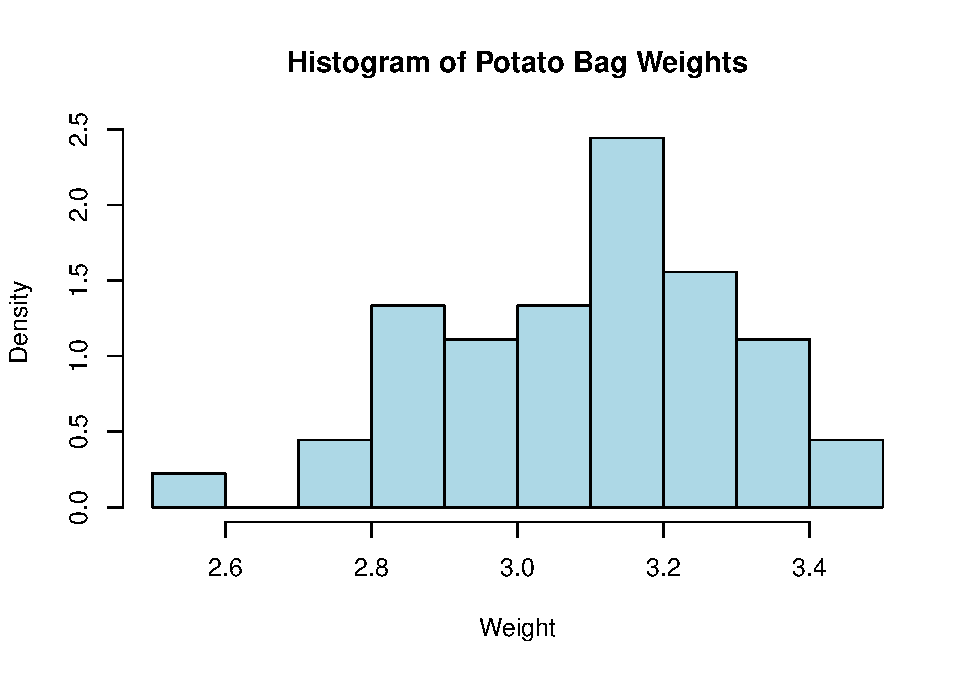
\includegraphics{final_work_stu_files/figure-latex/unnamed-chunk-3-1.pdf}

\newpage

\hypertarget{sampling-distribution-of-the-sample-mean-x_n}{%
\section{\texorpdfstring{Sampling distribution of the Sample Mean
\(X_{n}\)}{Sampling distribution of the Sample Mean X\_\{n\}}}\label{sampling-distribution-of-the-sample-mean-x_n}}

\begin{quote}
Find the expected value of the Sample Mean and its standard error.
\end{quote}

\(E[X_{n}] = \sum_{i=1}^{n}{x_i * P(x_i)} = 3.08\)

and standard error \(SD(X_{n}) = \sqrt{Var(x)} = 0.03\)

\vspace{2cm}

\begin{quote}
Which distribution follows the Sample Mean and why?
\end{quote}

\textbf{ANSWER:}\\
\vspace{2cm} \textgreater The sampling distribution of the sample mean
follows a normal distribution. This is based on the Central Limit
Theorem, which states that the distribution of the sample mean
approaches a normal distribution as the sample size increases.

\vspace{2cm}

\begin{quote}
Draw the curve supposing the original population has mean \(\mu = 3\)
and \(\sigma = 0.2\).
\end{quote}

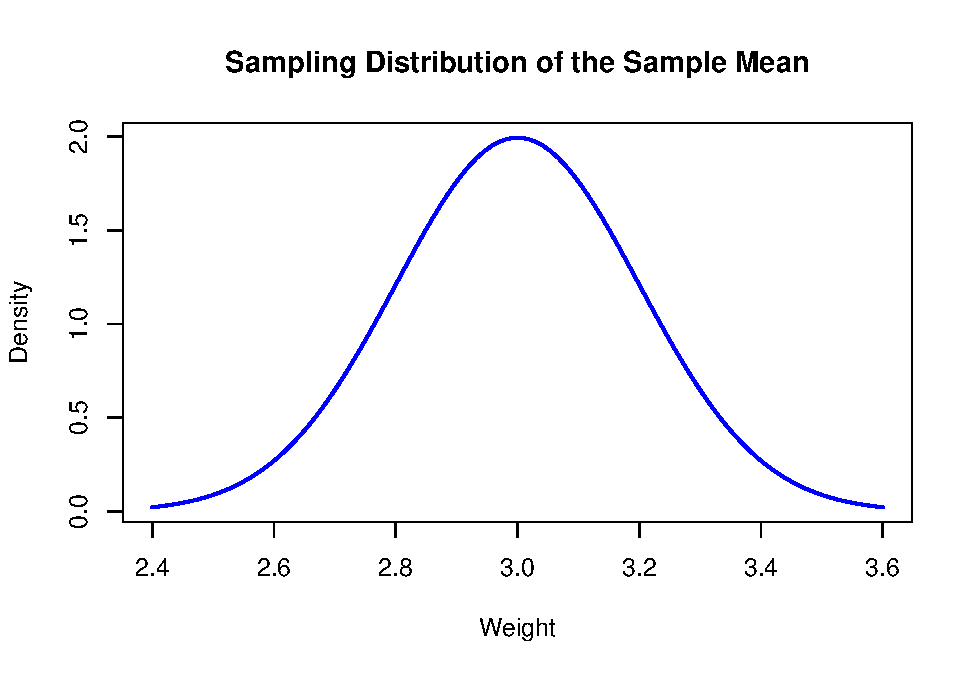
\includegraphics{final_work_stu_files/figure-latex/unnamed-chunk-5-1.pdf}

\newpage

\hypertarget{confidence-interval-for-the-mean}{%
\section{Confidence interval for the
mean}\label{confidence-interval-for-the-mean}}

\begin{quote}
\begin{enumerate}
\def\labelenumi{\arabic{enumi}.}
\tightlist
\item
  Which distribution do you use for finding the probability of the
  confidence interval? Write the formula for the scores.
\end{enumerate}
\end{quote}

\textbf{ANSWER:}\\
\vspace{2cm} We use the t-distribution to find the probability of the
confidence interval. The formula for the t-scores is:

\(t = \frac{\bar{x}-\mu}{\frac{s}{\sqrt{n}}}\)

\begin{quote}
\begin{enumerate}
\def\labelenumi{\arabic{enumi}.}
\setcounter{enumi}{1}
\tightlist
\item
  Find the corresponding quantiles using that distribution.
\end{enumerate}
\end{quote}

\textbf{ANSWER:} \vspace{2cm}

\begin{quote}
The value of the quantile corresponding to the significance level is
\(q =2.015368\)
\end{quote}

\begin{quote}
\begin{enumerate}
\def\labelenumi{\arabic{enumi}.}
\setcounter{enumi}{2}
\tightlist
\item
  And draw it in the graphic of the distribution.
\end{enumerate}
\end{quote}

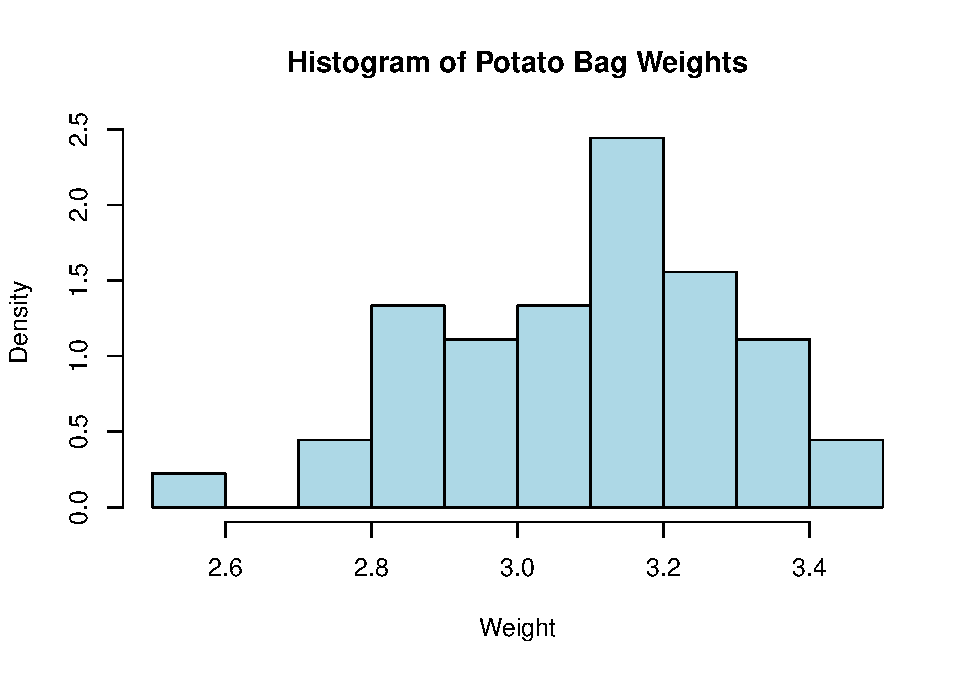
\includegraphics{final_work_stu_files/figure-latex/unnamed-chunk-7-1.pdf}

\vspace{2cm}

\begin{quote}
\begin{enumerate}
\def\labelenumi{\arabic{enumi}.}
\setcounter{enumi}{2}
\tightlist
\item
  Find the margin of error and the bounds of the interval.
\end{enumerate}
\end{quote}

\textbf{ANSWER:} \vspace{2cm}

\begin{quote}
The margin of error is \(0.058\)
\end{quote}

\begin{quote}
The bounds of the interval for the mean: \((3 , 3.2)\)
\end{quote}

\newpage

\hypertarget{test-the-following-hypothesis}{%
\section{Test the following
hypothesis}\label{test-the-following-hypothesis}}

\begin{quote}
To check if the machine is well calibrated, take a sample of 45 bags
filled with potatoes and count their weight. With this information,
\end{quote}

\begin{quote}
\begin{quote}
Does the engineer have reason to think the machine is poorly calibrated?
(Please use 5\% signication level).
\end{quote}
\end{quote}

\hypertarget{design-the-test}{%
\subsection{Design the test}\label{design-the-test}}

\begin{quote}
Define the null hypothesis and the alternative hypothesis
\end{quote}

\begin{quote}
The null hypothesis is \ldots{}``The machine is well calibrated.''
\end{quote}

\begin{quote}
The alternative hypothesis is \ldots{}``The machine is poorly
calibrated.''
\end{quote}

\begin{quote}
The significance level is \ldots{} 0.05
\end{quote}

\begin{quote}
\end{quote}

\hypertarget{find-the-corresponding-statistic-to-the-sample}{%
\subsection{Find the corresponding statistic to the
sample}\label{find-the-corresponding-statistic-to-the-sample}}

\begin{quote}
The statistic follows the \ldots. t-distribution
\end{quote}

\begin{quote}
The value of the corresponding statistic is ..\emph{\(FORMULA = 3.4\)}
\end{quote}

\hypertarget{find-the-critical-value-corresponding-to-the-significance-level}{%
\subsection{Find the critical value corresponding to the significance
level}\label{find-the-critical-value-corresponding-to-the-significance-level}}

\begin{quote}
The critical value is ..\emph{2.015368}
\end{quote}

\hypertarget{find-the-p-value}{%
\subsection{Find the p-value}\label{find-the-p-value}}

\begin{quote}
The p-value is \ldots{} \emph{\(P(T >= t | H_0) = 0.00157508\)}
\end{quote}

\hypertarget{make-the-decision}{%
\subsection{Make the decision}\label{make-the-decision}}

\begin{quote}
I reject the null hypothesis because the\ldots{} p-value is less than
the significance level.
\end{quote}

\hypertarget{type-of-errors}{%
\subsection{Type of errors}\label{type-of-errors}}

\begin{quote}
The value of Type I error is \ldots{}\emph{\(FORMULA = 0.05\)}
\end{quote}

\begin{quote}
The value of Type II error is \ldots{}\emph{\(FORMULA = 0.95\)}
\end{quote}

\end{document}
